\section{Aufbau}
\begin{frame}{Bodenstationen, {\small [gps.gov]}}
    \begin{figure}
        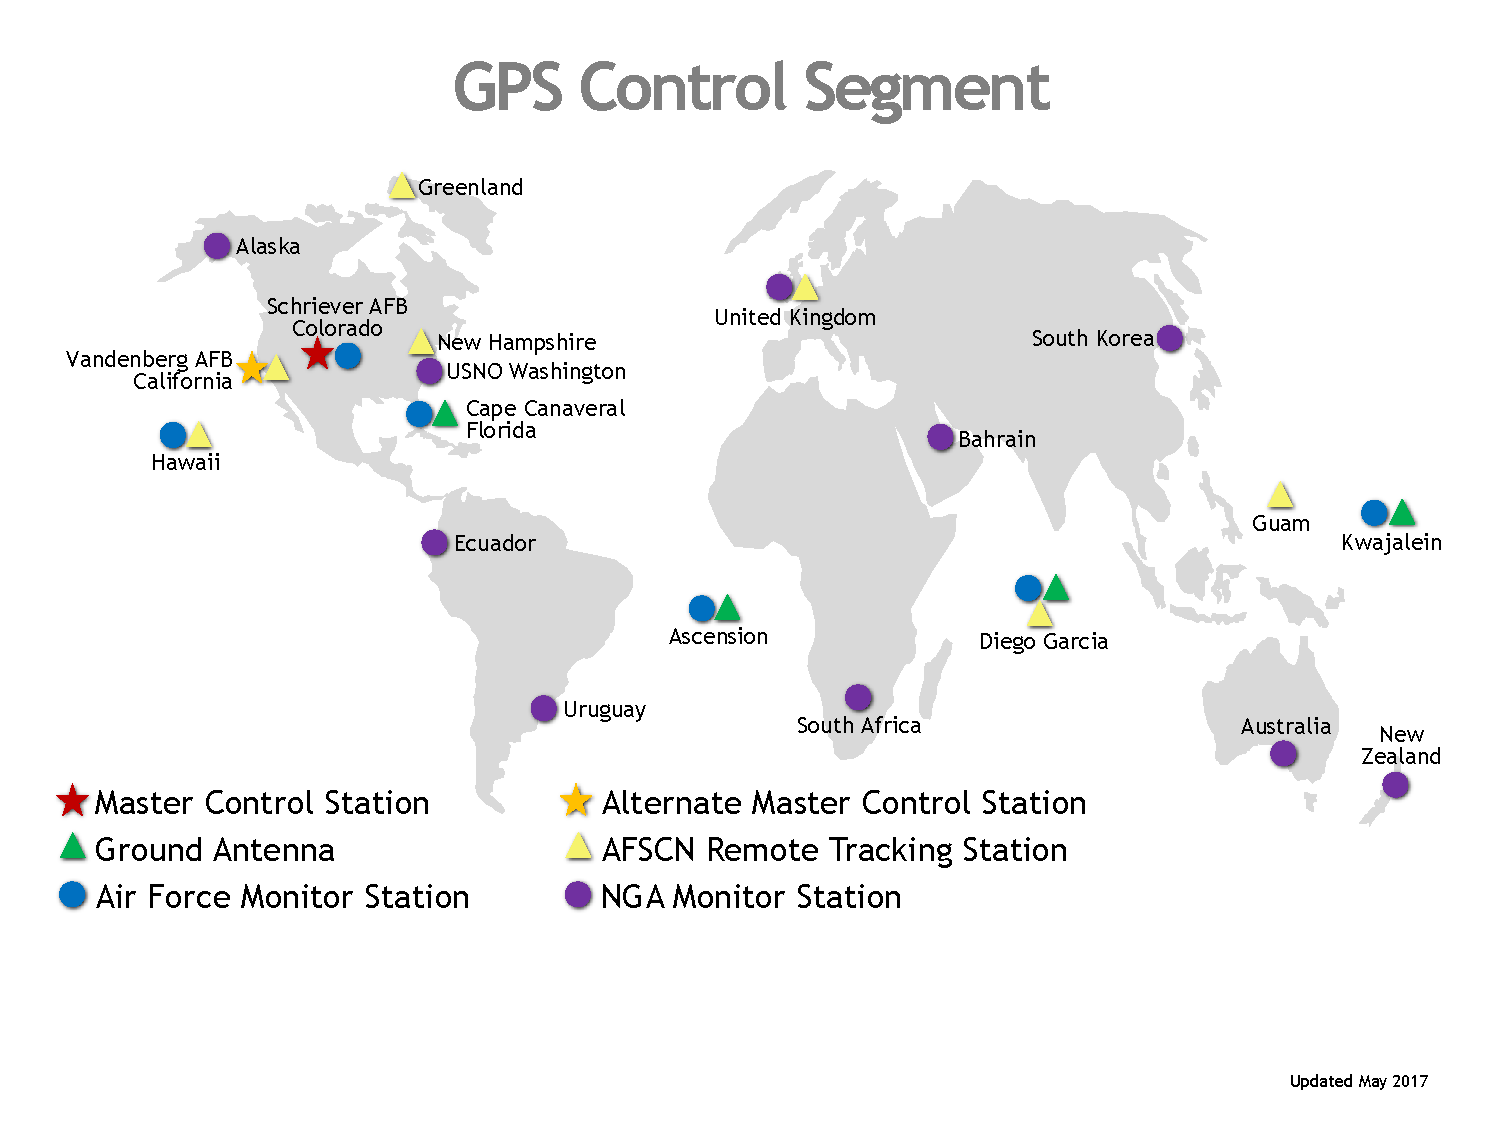
\includegraphics[height=1.1\textheight]{images/GPS-control-segment-map.pdf}
    \end{figure}
\end{frame}

\begin{frame}{Konstellation}
    \begin{columns}
        \begin{column}{0.5\textwidth}
            \begin{itemize}
                \item[Höhe:] \SI{20200}{\kilo\meter}
                \item[Umläufe:] 2 pro Tag
                \item[Orbitale:] 6, mit je 4 Satelliten
                \item[→] 4 Satelliten an jedem Ort sichtbar
                \item[2011:] Umpositionierung auf \textit{Expanable 24}\\mit 27 aktiven Satelliten
            \end{itemize}
        \end{column}
        \begin{column}{0.3\textwidth}
            \begin{figure}
                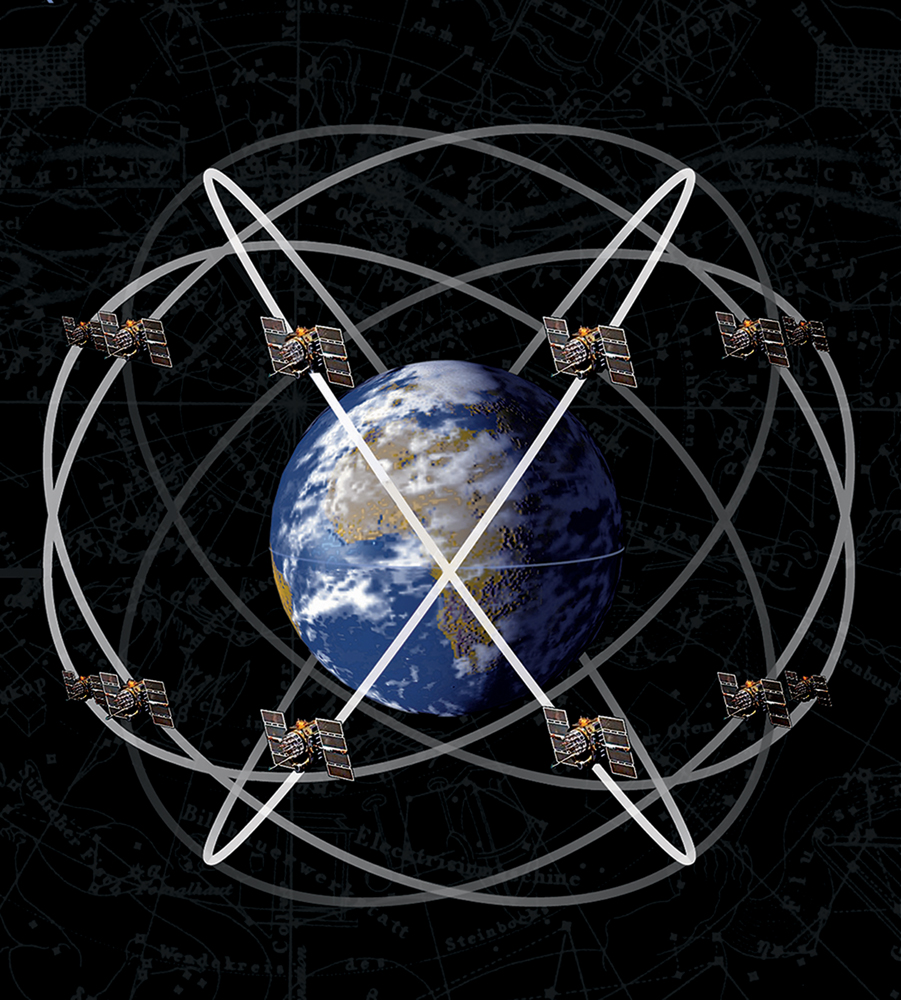
\includegraphics[width=\textwidth]{images/satelliten_schaubild.jpg}
            \end{figure}
            {\small [TimeAndNavigation]}
        \end{column}
    \end{columns}
\end{frame}

\begin{frame}{Die verschiedenen Satelliten im Überblick.}
    \begin{table}
        \begin{tabular}{c S[table-format=2.0] c S[table-format=2.1] c}
            \toprule
            {Generation} & {Aktiv} & {Start} & {\enquote{MHD}} & {Änderungen} \\
            \midrule
            Block IIA   &  1 & 1990-1997 & 7.5 & \\
            Block IIR   & 11 & 1997-2004 & 7.5 & Onboard Uhrüberwachung \\
            Block IIR-M &  7 & 2005-2009 & 7.5 & Mehr und stärkere M(ilitär)signale \\
            Block IIF   & 12 & 2010-2016 & 12  & neue Uhr, bessere Signalabstrahlung \\
            GPS III     &  0 & Dez 2018  & 15  & bessere Zuverlässigkeit, kein SA mehr \\
            GPS IIIF    &  0 & Dez 2018  & 15  & " , SAR kompatibel \\
            \bottomrule
        \end{tabular}
    \end{table}
    SA = selective Activity, ziviles GPS stören\\
    Grund: \textit{national security reasons}\\
    Abschaltung: 02.05.2000
\end{frame}

\begin{frame}{GPS-Satelliten}
    \begin{columns}
        \begin{column}{0.5\textwidth}
            \begin{figure}
                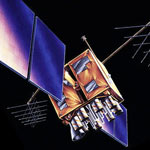
\includegraphics[width=0.5\textwidth]{images/IIR.jpg}
            \end{figure}
            \centering{Typ IIR}
        \end{column}
        \begin{column}{0.5\textwidth}
            \begin{figure}
                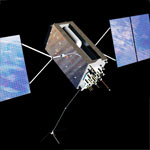
\includegraphics[width=0.5\textwidth]{images/IIIA.jpg}
            \end{figure}
            \centering{Typ III}
        \end{column}
    \end{columns}
\end{frame}
